\documentclass[../main.tex]{subfiles}

\graphicspath{{../images/}}

\begin{document}
\pagestyle{fancy}
\lhead{Lecture 7: 9/17/24}
\chead{Chapter 3}
\rhead{PHYS 421}

\section{Potentials}
\barh \vspace{1em}

\subsection{Laplace's Equation}

\subsubsection{Intro}
In principle, electrostatis is
\begin{align*}
    \vb E (\vb r) = \ke \int \frac{\vu\scriptr}{\scriptr^2} \rho(\vb r') \dd\tau', \quad \vb \scriptr = \vb r - \vb r'
\end{align*}
And simplifying with potential
\begin{align*}
    V(\vb r) = \ke \int \frac{\rho(\vb r')}{\scriptr} \dd \tau'
\end{align*}
So we often use Poisson's equation e.g.
\begin{align*}
    \laplacian V = -\frac{\rho}{\epsilon_0}
\end{align*}
Even better, Laplace's equation
\begin{align*}
    \boxed{\laplacian V = 0}
\end{align*}
or in Cartesian
\begin{align*}
    \laplacian V = \pdv[2]{V}{x} + \pdv[2]{V}{y} + \pdv[2]{V}{z} = 0
\end{align*}

\subsubsection{Start in 1D}
\begin{align*}
    \pdv[2]{V}{x} = 0 \implies V = mx + b
\end{align*}
where we have two undetermined constants $m$ \& $b$.
We can determine these constants by \textit{boundary conditions}.
\begin{itemize}
    \item e.g. $V(1) = 4 \quad V(5) = 0$; we get a line $V = -\frac{4}{5}x + 4$
\end{itemize}

\paragraph{Two features:}
\begin{enumerate}
    \item $V(x)$ is average of $V(x + a)$ and $V(x - a)$
    \begin{align*}
        V(x) = \frac{1}{2} \qt[V(x + a) + V(x - a)]
    \end{align*}
    \item \textbf{NO} local minima or maxima (no curvature!)
\end{enumerate}

\newpage
\subsubsection{On to 2D}
\begin{align*}
    \pdv[2]{V}{x} + \pdv[2]{V}{y} = 0 \qqtext{no general solution}
\end{align*}
and no requirement on the \# of constants.
But we can note common properties e.g. soap film on a wireframe assumes the same shape.
\begin{figure*}[ht]
    \centering
    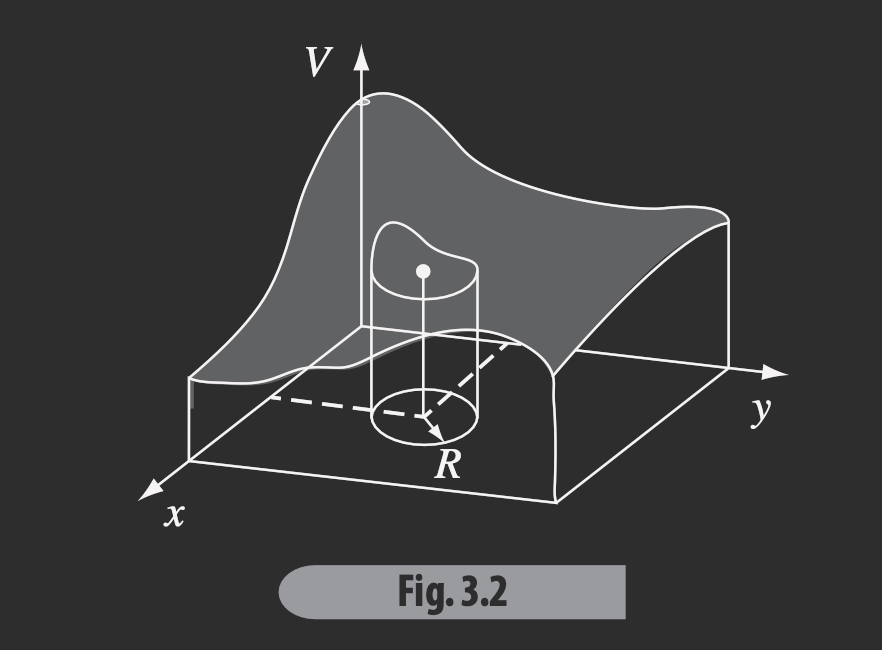
\includegraphics[width=0.3\linewidth]{fig3_2.png}
    \caption{}
    \label{fig:lecture3_2}
\end{figure*}
The solutions are called \textit{harmonic functions}:
\begin{enumerate}
    \item value $V(x,y)$ is average of nearby values; more precisely, for a circle of radius $R$ (Fig. \ref{fig:lecture3_2})
    \begin{align*}
        V(x,y) = \frac{1}{2\pi R} \oint V \dd\ell
    \end{align*}
    where $2\pi R$ is the circumference of the circle.
    \item \textbf{NO} local minima or maxima
\end{enumerate}

\subsubsection{In 3D}
\begin{align*}
    \laplacian V = 0
\end{align*}
Holds same properties as 2D:
\begin{enumerate}
    \item Average over spherical surface of radius $R$ centered at $\vb r$:
    \begin{align*}
        V(\vb r) = \frac{1}{4\pi R^2} \oint_S V \dd a
    \end{align*}
    where $4\pi R^2$ is the surface area of the sphere.
\end{enumerate}

\paragraph{Example:} Point charge outside sphere; The potential at $\dd a$
\begin{align*}
    V = \ke \frac{q}{\scriptr} 
\end{align*}
and from law of cosines 
\begin{align*}
    \scriptr^2 = z^2 + R^2 - 2rR\cos\theta
\end{align*}
so the average potential is
\begin{align*}
    V_\text{avg} &= \frac{q}{4\pi R^2} \ke \int \frac{R^2 \sin\theta \dd\theta \dd\phi}{\sqrt{z^2 + R^2 - 2zR\cos\theta}} \\
    &= \frac{q}{2zR} \ke \qt[z^2 + R^2 - 2zR\cos\theta]^{1/2} \eval_0^\pi \\
    &= \frac{q}{2zR} \ke \qt[(z + R) - (z - R)] \\
    &= \ke \frac{q}{z}
\end{align*}
which is just the potential of a point charge $q$ in the center of the sphere.

\paragraph{Question:} Is it possible to stably trap a charged particle using electrostatic forces alone? 

\paragraph{Answer} Earnshaw's theorem: A charged particle cannot be held in stable equilibrium by electrostatic forces alone.

\subsubsection{Boundary Conditions \& Uniqueness Theorem}

Laplace's eq requires boundary conditions (b.c.c)

\paragraph{1st uniqueness theorem:}

``Solutions to L's eq in volume $V$ is uniquely determined if potential is specied in surface $S$ bounding $V$.''

How is the solution unique?

Have solution in $V_1$ s.l.
\begin{align*}
    \laplacian V_1 = 0 \qqtext{also} \laplacian V_2 = 0
\end{align*}
Then
\begin{align*}
    V_3 \equiv \Delta V = V_1 - V_2
\end{align*}
which means
\begin{align*}
    \laplacian V_3 = \laplacian V_1 - \laplacian V_2 = 0 - 0 = 0
\end{align*}
thus
\begin{align*}
    \implies \laplacian V_1 &= \laplacian V_2 \\
    V_1 &= V_2
\end{align*}
We should emphasize that $V_1$ defined on the boundary $S$ is also the same b.c.s as $V_2$ while $V_3$ on the boundary equals zero.
That is $V_3$ is zero everywhere in space.

\subsubsection{2nd uniqueness theorem (conductors):}

``In a volume $V$ surrounded by conductors, and containing a specifed charge density $\rho$,
then the $\vb E$ field is uniquely determined if the total charge on each conductor is given.''

``This proof was not easy'' - Griffiths

\paragraph{Example:} Connecting two pairs of opposite charges with a conductor;
what is the final charge config and E-field?

\paragraph{Answer:} $\vb E = 0$ everywhere. The total charge of each conductor is zero.

\subsubsection{Boundary conditions pt. II}

(Griffiths 2.3.5 pg 85) Given a sheet of charge $\sigma = Q/ A$ and using the Gaussian pillbox method 
\begin{align*}
    \oint \vb E \cdot \dd\vb a &= \frac{q_\text{enc}}{\epsilon_0} \\
    E_a A - E_b A &= \sigma \frac{A}{\epsilon_0} \\
    E_a - E_b &= \frac{\sigma}{\epsilon_0}
\end{align*}

For the same surface we know that
\begin{align*}
    \curl \vb E = \oint \vb E \cdot \dd\ell = 0
\end{align*}
So going around the loop we have
\begin{align*}
    E_a \ell - E_b \ell &= 0 \\
    E_a &= E_b
\end{align*}

\newpage
\subsection{Method of Images}
\lhead{Lecture 8: 9/19/24}

$\laplacian V = -\rho/\epsilon_0$ \textit{is} electrostatics. AND when we have $\laplacian V = 0$, Uniqueness theorems tell us there is a solution,
but doesn't tell us how to find it\dots thus we have a set of ``easily'' solvable problems.

\subsubsection{Classic image problem:}

``Ground'' is infinite conducting plane $V = 0$ at $z = 0$. For a charge $q$ at $z = d$ what is the potential in $z > 0$?
We know that the point charge will induce a charge on the plane which will effect the electic potential in the region $z > 0$.
% fig3_10
\begin{figure*}[ht]
    \centering
    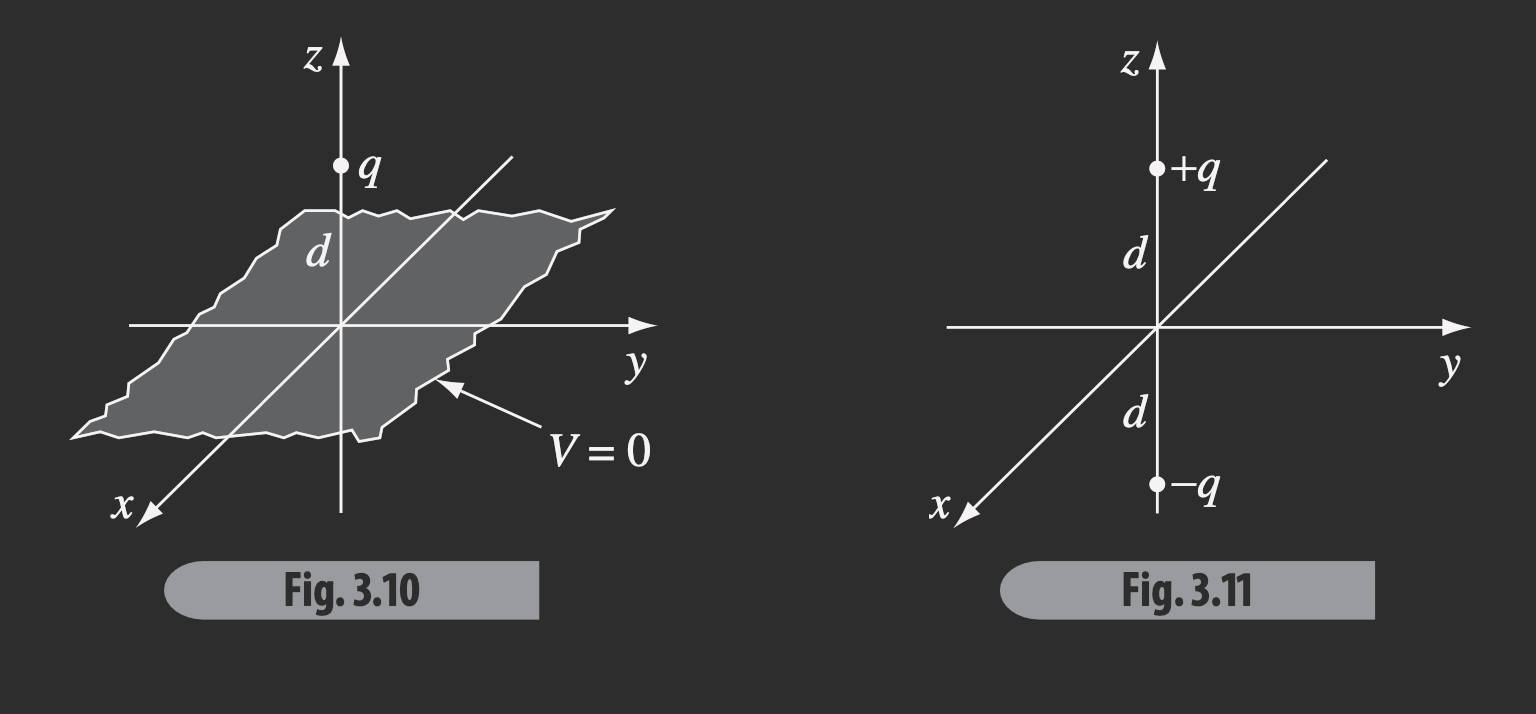
\includegraphics[width=0.5\linewidth]{fig3_10.png}
    \caption{}
    \label{fig:lecture3_10}
\end{figure*}

\paragraph{GOAL: } solve $\laplacian V = -\rho/\epsilon_0$ for $z \geq 0$ 
with $+q$ at $(0,0,d)$ subject to boundary conditions (b.c.s)
\begin{enumerate}
    \item $V(z=0) = 0$ 
    \item $V \to 0$ for far away
\end{enumerate}
The next step is to replace the conducting plane with an equivalent charge $-q$ at $z = -d$.

NOTE: We only care about $z \geq 0$ and ignore $z < 0$ region; furthermore, the potential below the plane should be zero as the boundary of the plane sort of ``wraps'' around the charge

Thus the solution is a superposition of charges
\begin{align*}
    V = \ke \qt[\frac{q}{\sqrt{x^2 + y^2 + (z-d)^2}} - \frac{q}{\sqrt{x^2 + y^2 + (z+d)^2}}]
\end{align*}
we can see that in the replacement problem, the region below the grounded plane is nonzero which is different from the real problem which is why we ignore it!

\subsubsection{Induced surface charge} 

What is $\sigma$? Recall on the sheet $\sigma$ we have a field
\begin{align*}
    \vb E_\textrm{ab} - \vb E_\textrm{be} = \frac{\sigma}{\epsilon_0} \vu n
\end{align*}
where the $\vu n$ tells us that we are dealing with the perpendicular planes; thus the same eq
\begin{align*}
    \grad V_\text{ab} - \grad V_\text{be} = -\frac{\sigma}{\epsilon_0} \vu n \implies \vb E = -\grad V
\end{align*}
We can infer that
\begin{align*}
    \pdv{V_a}{n} - \cancel{\pdv{V_b}{n}} = -\frac{\sigma}{\epsilon_0}
\end{align*}
since anything below the plane is zero from the previous example. We know have
\begin{align*}
    \pdv{V_a}{z} \eval_{z\to 0} &= \ke \qt[-\frac{q(z-d)}{(x^2 + y^2 + (z-d)^2)^{3/2}} + \frac{q(z+d)}{(x^2 + y^2 + (z+d)^2)^{3/2}}] \eval_{z\to 0}
\end{align*}
So
\begin{align*}
    \sigma = -\frac{1}{2\pi} \frac{qd}{(x^2 + y^2 + d^2)^{3/2}}
\end{align*}
We can check that the total induced charge in the plane is infact
\begin{align*}
    Q = \int_0^{2\pi} \int_0^\infty \sigma  r\dd r \dd\phi = - q
\end{align*}
where $r^2 = x^2 + y^2$.

This charge comes from the reservoir of charge given by ground.

\begin{figure*}[ht]
    \centering
    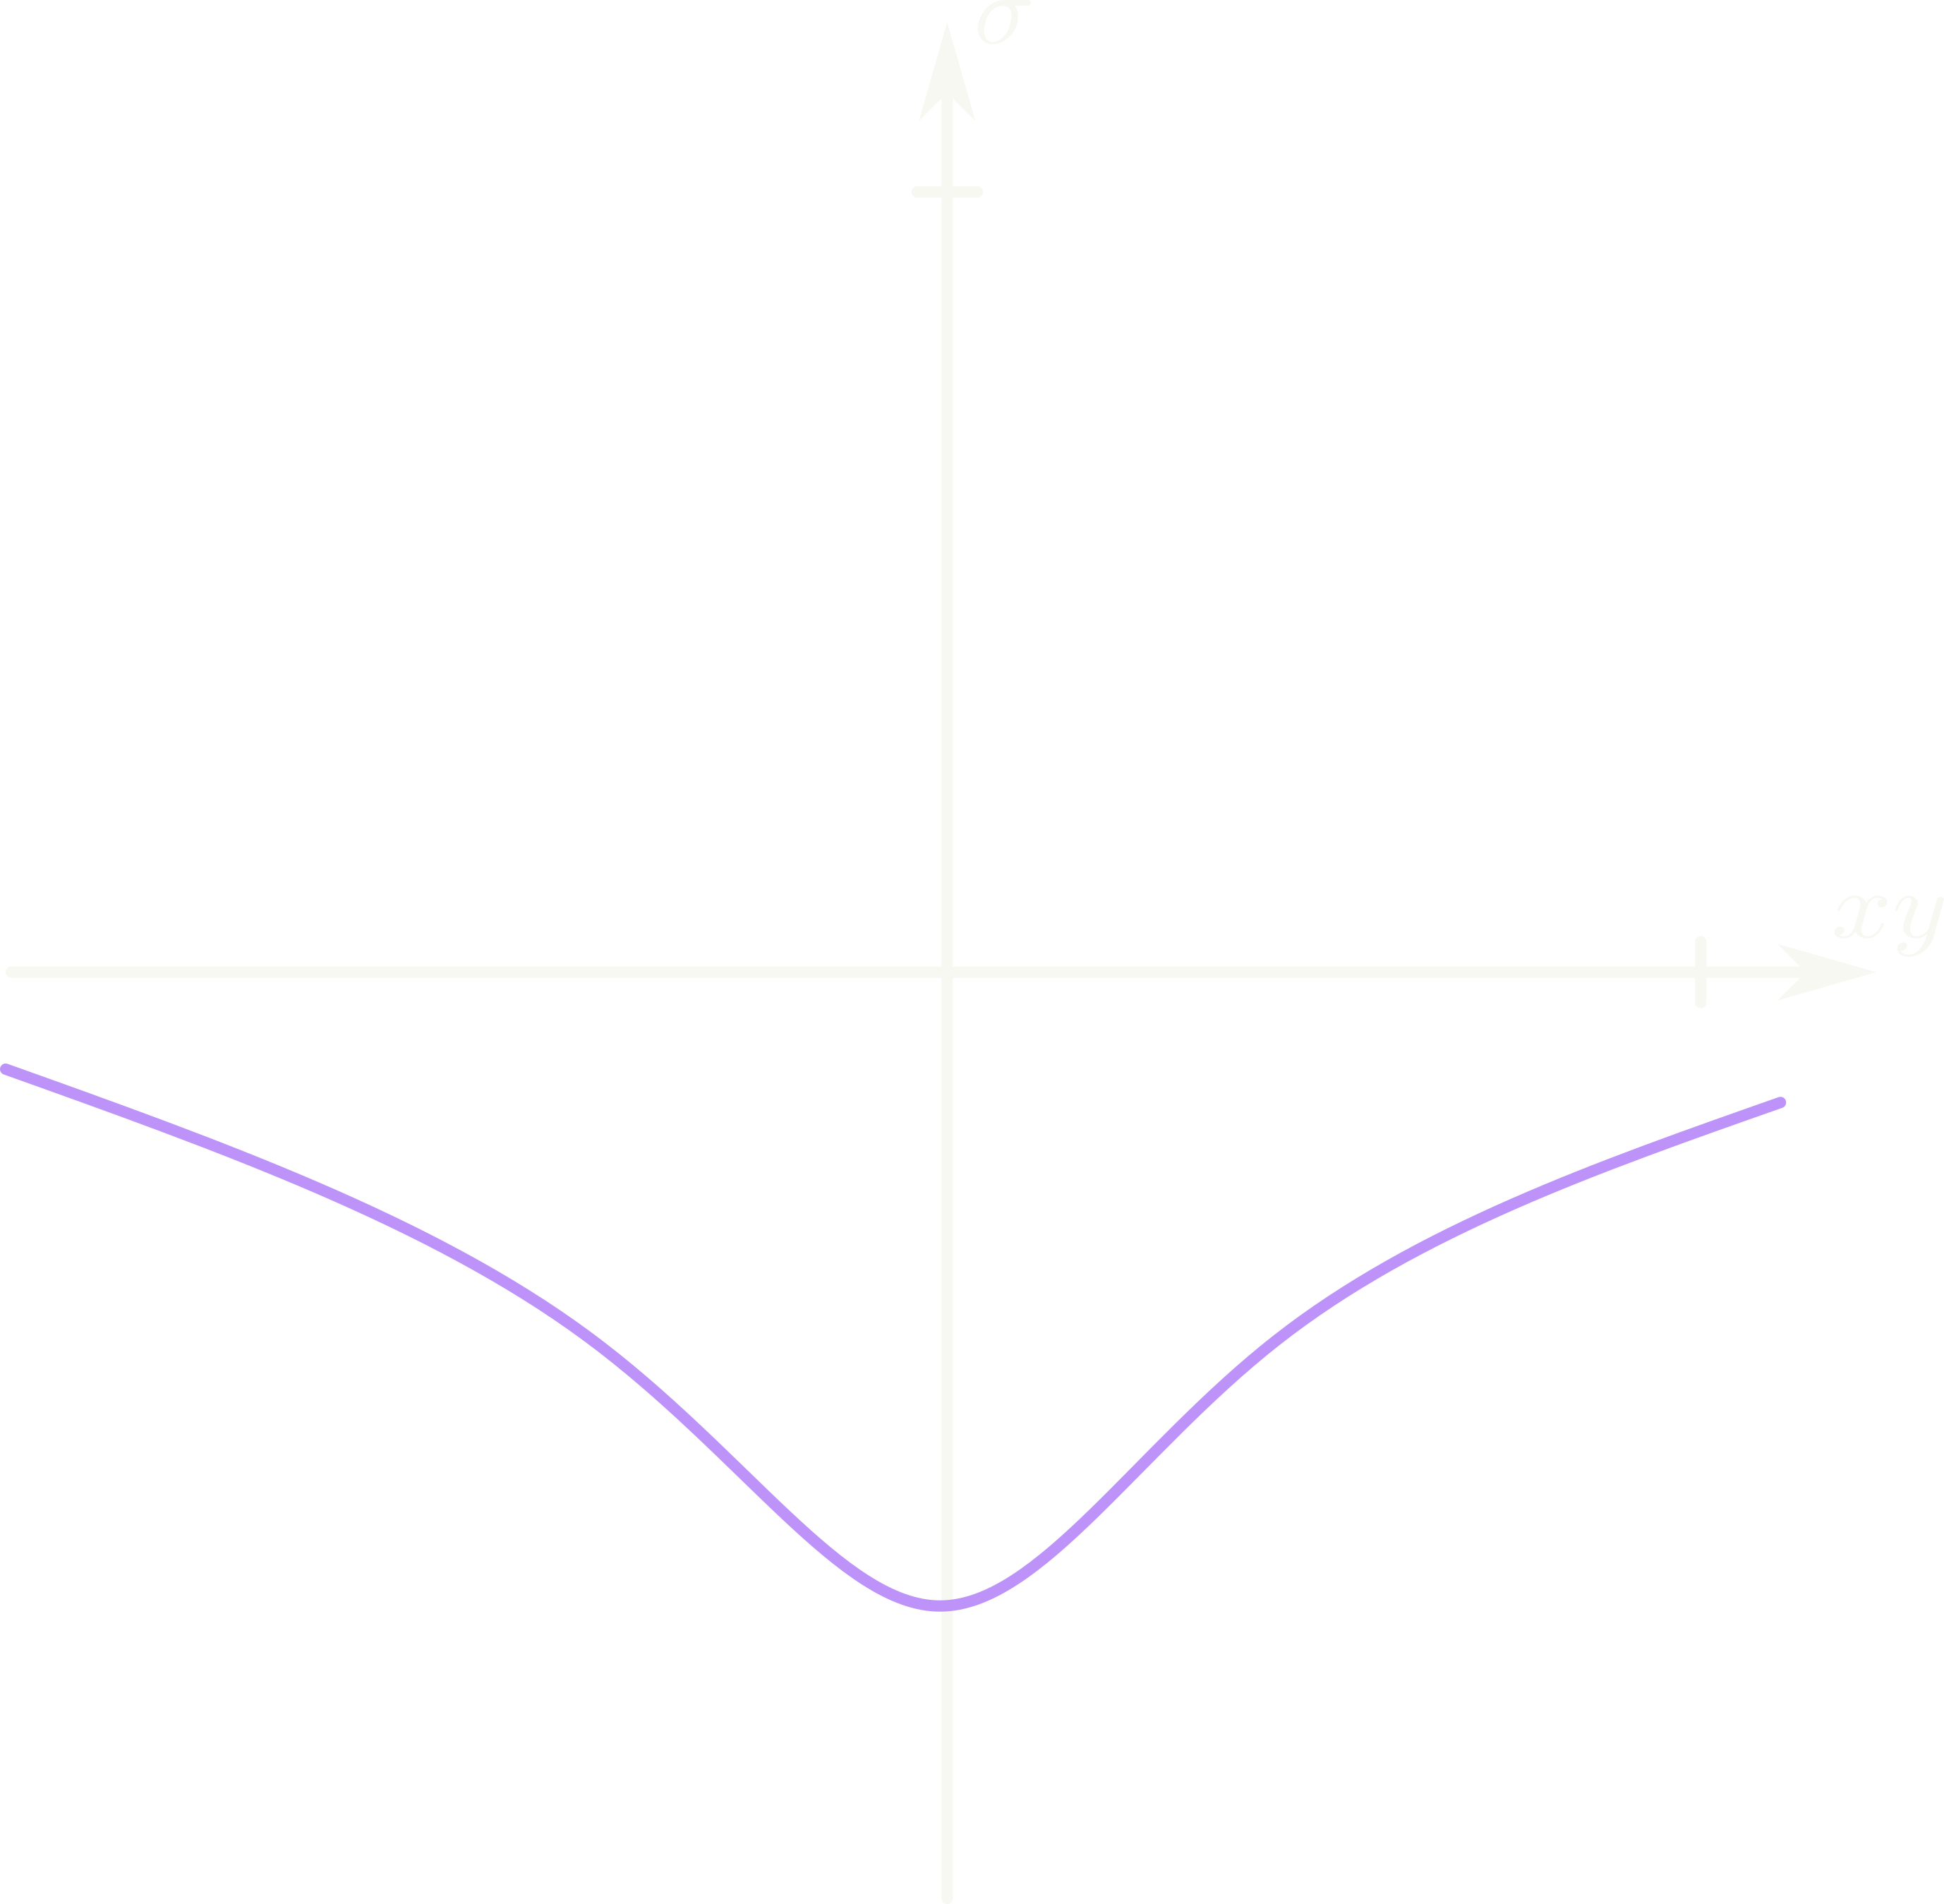
\includegraphics[width=0.3\linewidth]{fig3_11.png}
    \caption{Just a cool graph of $xy$ vs $\sigma$}
    \label{fig:lecture3_11}
\end{figure*}

\subsubsection{Force and energy}

Calcuating the force of attraction because of the negative induced charge:
\begin{align*}
    F = qE = \ke \frac{q^2}{(2d)^2} (-\vu z)
\end{align*}
Naively, we calculate the energy/work done as
\begin{align*}
    W = -\ke \frac{q^2}{2d} \quad (=q \Delta V)
\end{align*}
but we only have a single charge and the total work is half of this value
\begin{align*}
    W = -\ke \frac{q^2}{4d}
\end{align*}
This is because the ideal conductor requires no work to build up a charge distribution $\sigma$.

\newpage
\subsection{Seperation of Variables}

\begin{figure*}[ht]
    \centering
    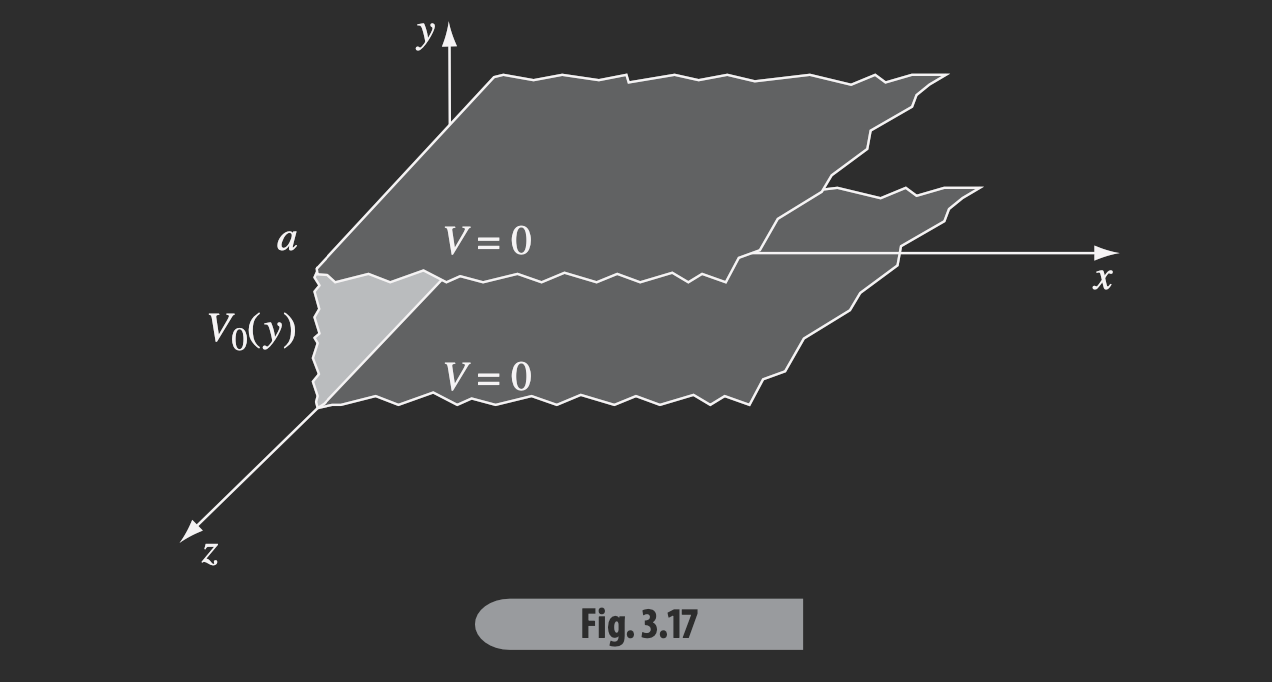
\includegraphics[width=0.5\linewidth]{fig3_17.png}
    \caption{3 planes where top and bottom are grounded and the middle is at $V_0(y)$}
    \label{fig:lecture3_17}
\end{figure*}

Find potential $V$ in $x > 0$, $0< y < a$, $-\infty < z < \infty$:

This is a 2D problem $V\to V(x,y)$

No change in $V \to \laplacian V = 0 = \pdv[2]{V}{x} + \pdv[2]{V}{y}$. 

From b.c.s
\begin{enumerate}
    \item $V(y=0) = 0$
    \item $V(y=a) = 0$
    \item $V(x=0) = V_0(y)$
    \item $V(x\to\infty) = 0$
\end{enumerate}

PROPOSE: $V(x,y) = X(x)Y(y)$
\begin{align*}
    \laplacian V &= Y\pdv[2]{X}{x} + X\pdv[2]{Y}{y} = 0 \\
    \frac{\laplacian V}{V} = \frac{1}{X} \pdv[2]{X}{x} + \frac{1}{Y} \pdv[2]{Y}{y} &= 0
\end{align*}
\end{document}